% Created by tikzDevice version 0.10.1 on 2018-02-09 14:36:33
% !TEX encoding = UTF-8 Unicode
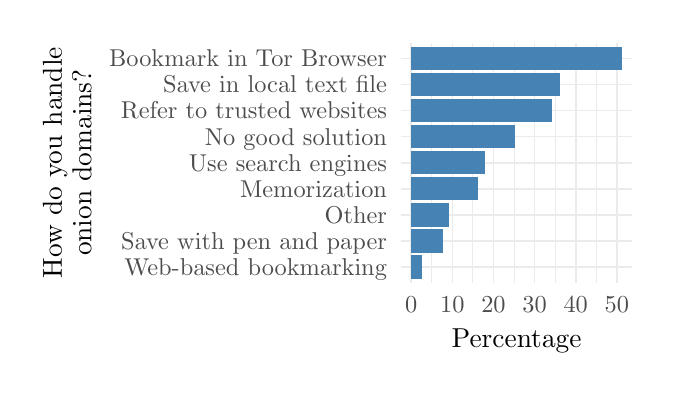
\begin{tikzpicture}[x=1pt,y=1pt]
\definecolor{fillColor}{RGB}{255,255,255}
\path[use as bounding box,fill=fillColor,fill opacity=0.00] (0,0) rectangle (224.04,122.86);
\begin{scope}
\path[clip] (134.78, 30.77) rectangle (218.54,117.36);
\definecolor{drawColor}{gray}{0.92}

\path[draw=drawColor,line width= 0.3pt,line join=round] (146.02, 30.77) --
	(146.02,117.36);

\path[draw=drawColor,line width= 0.3pt,line join=round] (160.88, 30.77) --
	(160.88,117.36);

\path[draw=drawColor,line width= 0.3pt,line join=round] (175.74, 30.77) --
	(175.74,117.36);

\path[draw=drawColor,line width= 0.3pt,line join=round] (190.61, 30.77) --
	(190.61,117.36);

\path[draw=drawColor,line width= 0.3pt,line join=round] (205.47, 30.77) --
	(205.47,117.36);

\path[draw=drawColor,line width= 0.6pt,line join=round] (134.78, 36.42) --
	(218.54, 36.42);

\path[draw=drawColor,line width= 0.6pt,line join=round] (134.78, 45.83) --
	(218.54, 45.83);

\path[draw=drawColor,line width= 0.6pt,line join=round] (134.78, 55.24) --
	(218.54, 55.24);

\path[draw=drawColor,line width= 0.6pt,line join=round] (134.78, 64.65) --
	(218.54, 64.65);

\path[draw=drawColor,line width= 0.6pt,line join=round] (134.78, 74.07) --
	(218.54, 74.07);

\path[draw=drawColor,line width= 0.6pt,line join=round] (134.78, 83.48) --
	(218.54, 83.48);

\path[draw=drawColor,line width= 0.6pt,line join=round] (134.78, 92.89) --
	(218.54, 92.89);

\path[draw=drawColor,line width= 0.6pt,line join=round] (134.78,102.30) --
	(218.54,102.30);

\path[draw=drawColor,line width= 0.6pt,line join=round] (134.78,111.71) --
	(218.54,111.71);

\path[draw=drawColor,line width= 0.6pt,line join=round] (138.58, 30.77) --
	(138.58,117.36);

\path[draw=drawColor,line width= 0.6pt,line join=round] (153.45, 30.77) --
	(153.45,117.36);

\path[draw=drawColor,line width= 0.6pt,line join=round] (168.31, 30.77) --
	(168.31,117.36);

\path[draw=drawColor,line width= 0.6pt,line join=round] (183.17, 30.77) --
	(183.17,117.36);

\path[draw=drawColor,line width= 0.6pt,line join=round] (198.04, 30.77) --
	(198.04,117.36);

\path[draw=drawColor,line width= 0.6pt,line join=round] (212.90, 30.77) --
	(212.90,117.36);
\definecolor{fillColor}{RGB}{70,130,180}

\path[fill=fillColor] (138.58, 32.18) rectangle (142.54, 40.66);

\path[fill=fillColor] (138.58, 41.60) rectangle (150.15, 50.07);

\path[fill=fillColor] (138.58, 51.01) rectangle (152.13, 59.48);

\path[fill=fillColor] (138.58, 60.42) rectangle (162.84, 68.89);

\path[fill=fillColor] (138.58, 69.83) rectangle (165.10, 78.30);

\path[fill=fillColor] (138.58, 79.24) rectangle (176.10, 87.71);

\path[fill=fillColor] (138.58, 88.65) rectangle (189.36, 97.12);

\path[fill=fillColor] (138.58, 98.07) rectangle (192.45,106.54);

\path[fill=fillColor] (138.58,107.48) rectangle (214.73,115.95);
\end{scope}
\begin{scope}
\path[clip] (  0.00,  0.00) rectangle (224.04,122.86);
\definecolor{drawColor}{gray}{0.30}

\node[text=drawColor,anchor=base east,inner sep=0pt, outer sep=0pt, scale=  0.88] at (129.83, 33.39) {Web-based bookmarking};

\node[text=drawColor,anchor=base east,inner sep=0pt, outer sep=0pt, scale=  0.88] at (129.83, 42.80) {Save with pen and paper};

\node[text=drawColor,anchor=base east,inner sep=0pt, outer sep=0pt, scale=  0.88] at (129.83, 52.21) {Other};

\node[text=drawColor,anchor=base east,inner sep=0pt, outer sep=0pt, scale=  0.88] at (129.83, 61.62) {Memorization};

\node[text=drawColor,anchor=base east,inner sep=0pt, outer sep=0pt, scale=  0.88] at (129.83, 71.04) {Use search engines};

\node[text=drawColor,anchor=base east,inner sep=0pt, outer sep=0pt, scale=  0.88] at (129.83, 80.45) {No good solution};

\node[text=drawColor,anchor=base east,inner sep=0pt, outer sep=0pt, scale=  0.88] at (129.83, 89.86) {Refer to trusted websites};

\node[text=drawColor,anchor=base east,inner sep=0pt, outer sep=0pt, scale=  0.88] at (129.83, 99.27) {Save in local text file};

\node[text=drawColor,anchor=base east,inner sep=0pt, outer sep=0pt, scale=  0.88] at (129.83,108.68) {Bookmark in Tor Browser};
\end{scope}
\begin{scope}
\path[clip] (  0.00,  0.00) rectangle (224.04,122.86);
\definecolor{drawColor}{gray}{0.30}

\node[text=drawColor,anchor=base,inner sep=0pt, outer sep=0pt, scale=  0.88] at (138.58, 19.76) {0};

\node[text=drawColor,anchor=base,inner sep=0pt, outer sep=0pt, scale=  0.88] at (153.45, 19.76) {10};

\node[text=drawColor,anchor=base,inner sep=0pt, outer sep=0pt, scale=  0.88] at (168.31, 19.76) {20};

\node[text=drawColor,anchor=base,inner sep=0pt, outer sep=0pt, scale=  0.88] at (183.17, 19.76) {30};

\node[text=drawColor,anchor=base,inner sep=0pt, outer sep=0pt, scale=  0.88] at (198.04, 19.76) {40};

\node[text=drawColor,anchor=base,inner sep=0pt, outer sep=0pt, scale=  0.88] at (212.90, 19.76) {50};
\end{scope}
\begin{scope}
\path[clip] (  0.00,  0.00) rectangle (224.04,122.86);
\definecolor{drawColor}{RGB}{0,0,0}

\node[text=drawColor,anchor=base,inner sep=0pt, outer sep=0pt, scale=  0.99] at (176.66,  7.44) {Percentage};
\end{scope}
\begin{scope}
\path[clip] (  0.00,  0.00) rectangle (224.04,122.86);
\definecolor{drawColor}{RGB}{0,0,0}

\node[text=drawColor,rotate= 90.00,anchor=base,inner sep=0pt, outer sep=0pt, scale=  0.99] at ( 12.32, 74.07) {How do you handle};

\node[text=drawColor,rotate= 90.00,anchor=base,inner sep=0pt, outer sep=0pt, scale=  0.99] at ( 23.01, 74.07) {onion domains?};
\end{scope}
\end{tikzpicture}
